%%%%%%%%%%%%%%%%%%%%%%%%%%%%%%%%%%%%%%%%%%%%%%%%%%%%%%%%%%%%
%%  This Beamer template was created by Cameron Bracken.
%%  Anyone can freely use or modify it for any purpose
%%  without attribution.
%%
%%  Last Modified: January 9, 2009
%%

\documentclass[xcolor=x11names,compress]{beamer}

%% General document %%%%%%%%%%%%%%%%%%%%%%%%%%%%%%%%%%
\usepackage{graphicx}

\usepackage[mathscr]{eucal}
\usepackage{amsfonts}
\usepackage{amsmath}
\usepackage{amsthm}
\usepackage{amssymb}
\usepackage{latexsym}
\usepackage{svg}
\include{svg.dtx}
\usepackage{graphicx}
\usepackage{color}
\usepackage[noadjust]{cite}
\usepackage{epsfig}
\usepackage{tikz-cd}
\usepackage{float}
\usepackage{soul}
\setuldepth{Berlin}
\allowdisplaybreaks

\let\nc\newcommand
\let\rnc\renewcommand
\nc{\la}{\label}
\def\bg{\begin}
\nc{\End}{{\rm{End}}}
\nc{\Hom}{{\rm{Hom}}}
\newcommand{\id}{{\rm{id}}}
\newcommand{\Tr}{{\rm{Tr}}}
\newcommand{\tr}{{\rm{tr}}}
\newcommand{\cn}{\mathrm{cn}}
\newcommand{\cl}{\mathrm{cl}}
\newcommand{\Ker}{{\rm{Ker}}}
\newcommand{\ev}{{\rm{ev}}}
\newcommand{\im}{{\rm{Im}}}
\newcommand{\interior}{{\rm{int}}}
\newcommand{{\scrc}}{\mathscr{C}}
\newcommand{{\sfc}}{\mathsf{C}}
\newcommand{{\sfr}}{\mathsf{R}}
\newcommand{{\sfskein}}{\mathsf{Skein}}
\newcommand{{\sft}}{\mathsf{T}}
\newcommand{{\sfd}}{\mathsf{D}}
\newcommand{{\sfh}}{\mathsf{H}}
\newcommand{{\cs}}{\mathcal{S}}
\newcommand{{\cc}}{\mathcal{C}}
\newcommand{{\ct}}{\mathcal{T}}
\newcommand{{\ca}}{\mathcal{A}}
\newcommand{{\ck}} {\mathcal{K}}
\newcommand{{\cd}} {\mathcal{D}}
\newcommand{{\ch}} {\mathcal{H}}
\newcommand{\ci}{\mathcal{I}}
\newcommand{\xx}{{\mathbf{x}}}
\newcommand{\yy}{{\mathbf{y}}}
\newcommand{\zz}{{\mathbf{z}}}
\newcommand{\aab}{{\mathbf{a}}}
\newcommand{\bb}{{\mathbf{b}}}
\newcommand{\SL}{\mathrm{SL}}
\newcommand{\HH}{\mathrm{HH}}
\newcommand{\E}{\mathcal{E}}
\newcommand{\GL}{\mathrm{GL}}
\newcommand{\N}{\mathbb{N}}
\newcommand{{\Z}}{\mathbb{Z}}
\newcommand{\Q}{\mathbb{Q}}
\newcommand{\C}{\mathbb{C}}
\newcommand{\sk}{\mathrm{Sk}}
\newcommand{\fg}{\mathfrak{g}}
\newcommand{\fa}{\mathfrak{a}}
\newcommand{\fb}{\mathfrak{b}}
\newcommand{\AP}[1]{{\color{blue} * #1}}
\newcommand{\pic}[2][3]{{\,\vcenter{\hbox{\includegraphics[width= #1 cm]{#2}}}}}

\tikzset{
    invisible/.style={opacity=0},
    visible on/.style={alt={#1{}{invisible}}},
    alt/.code args={<#1>#2#3}{%
      \alt<#1>{\pgfkeysalso{#2}}{\pgfkeysalso{#3}}%
  }
}
%%%%%%%%%%%%%%%%%%%%%%%%%%%%%%%%%%%%%%%%%%%%%%%%%%%%%%


%% Beamer Layout %%%%%%%%%%%%%%%%%%%%%%%%%%%%%%%%%%
\useoutertheme[subsection=false,shadow]{miniframes}
\useinnertheme{default}
\usefonttheme{serif}
\usepackage{palatino}

\setbeamerfont{title like}{shape=\scshape}
\setbeamerfont{frametitle}{shape=\scshape}

\setbeamercolor*{lower separation line head}{bg=DeepSkyBlue4} 
\setbeamercolor*{normal text}{fg=black,bg=white} 
\setbeamercolor*{alerted text}{fg=red} 
\setbeamercolor*{example text}{fg=black} 
\setbeamercolor*{structure}{fg=black} 

\setbeamercolor{block title}{use=structure,fg=white,bg=DeepSkyBlue4}
\setbeamercolor{block body}{parent=normal text,use=block title,bg=block title.bg!10!bg}
 
\setbeamercolor*{palette tertiary}{fg=black,bg=black!10} 
\setbeamercolor*{palette quaternary}{fg=black,bg=black!10} 

\renewcommand{\(}{\begin{columns}}
\renewcommand{\)}{\end{columns}}
\newcommand{\<}[1]{\begin{column}{#1}}
\renewcommand{\>}{\end{column}}

\beamertemplatenavigationsymbolsempty 
%%%%%%%%%%%%%%%%%%%%%%%%%%%%%%%%%%%%%%%%%%%%%%%%%%




\begin{document}


%%%%%%%%%%%%%%%%%%%%%%%%%%%%%%%%%%%%%%%%%%%%%%%%%%%%%%
%%%%%%%%%%%%%%%%%%%%%%%%%%%%%%%%%%%%%%%%%%%%%%%%%%%%%%
\section{\scshape Introduction}
\begin{frame}
\title{Dubrovnik Skein Theory and Power Sum Elements}
%\subtitle{SUBTITLE}
\author{
	Alexander Pokorny\\
	{\it University of California, Riverside}\\
}
\date{
	$\pic[2]{wikipedia_trefoil.eps}$
	\\
	\vspace{1cm}
	\today
}
\titlepage
\end{frame}

%%%%%%%%%%%%%%%%%%%%%%%%%%%%%%%%%%%%%%%%%%%%%%%%%%%%%%
%%%%%%%%%%%%%%%%%%%%%%%%%%%%%%%%%%%%%%%%%%%%%%%%%%%%%%
\begin{frame}{Introduction}
\tableofcontents
\end{frame}

%%%%%%%%%%%%%%%%%%%%%%%%%%%%%%%%%%%%%%%%%%%%%%%%%%%%%%
%%%%%%%%%%%%%%%%%%%%%%%%%%%%%%%%%%%%%%%%%%%%%%%%%%%%%%
\section{\scshape Background}
\begin{frame}{(Framed) Link Invariants}
\begin{center}
\[\pic[2]{wikipedia_trefoil_mirror.eps} \qquad \qquad \quad \, \pic[0.7]{maybe_equal.eps} \, \qquad \qquad \quad \pic[2]{wikipedia_trefoil.eps}\] \pause
\[\pic[0.5]{longmapsto.eps} \qquad \quad \textrm{Dubrovnik Polynomial} \,\quad \qquad \pic[0.5]{longmapsto.eps} \]
\[\pic[2]{p_1.eps} \qquad \qquad \quad \pic[0.7]{neq.eps} \,\,\quad \qquad \qquad \pic[2]{p_2.eps}\]
\end{center}
\vspace{2cm}

\end{frame}

%%%%%%%%%%%%%%%%%%%%%%%%%%%%%%%%%%%%%%%%%%%%%%%%%%%%%%
%%%%%%%%%%%%%%%%%%%%%%%%%%%%%%%%%%%%%%%%%%%%%%%%%%%%%%
\begin{frame}{Dubrovnik Skein Relations}

\begin{align}
&\pic[1.5]{poscross.eps} = \pic[1.5]{negcross.eps} + (s-s^{-1}) \left( \pic[1.5]{idresolution.eps} - \pic[1.5]{capcupresolution.eps} \right) \\ \vspace{1cm}
&\pic[1.5]{vh.eps} = v \pic[1.5]{frameresolution.eps}\\ \vspace{1cm}
&\pic[1.5]{unknot.eps} = \left( 1 - \frac{v-v^{-1}}{s-s^{-1}} \right) \pic[1.5]{empty.eps} 
\end{align} \pause
\makebox[\linewidth][l]{\rule{11cm}{0.4pt}}
$\pic[1.6]{wikipedia_trefoil_circ.eps} = \pic[1.6]{wikipedia_trefoil_circ1.eps} + (s-s^{-1}) \left( \pic[1.6]{wikipedia_trefoil_circ2.eps} - \pic[1.6]{wikipedia_trefoil_circ3.eps} \right)$
\end{frame}

%%%%%%%%%%%%%%%%%%%%%%%%%%%%%%%%%%%%%%%%%%%%%%%%%%%%%%
%%%%%%%%%%%%%%%%%%%%%%%%%%%%%%%%%%%%%%%%%%%%%%%%%%%%%%
\begin{frame}{Skein Modules}
\ul{Observation:} Skein relations are defined locally. \\ \pause
\ul{Consequence:} May impose skein relations on tangles in $\qquad\qquad\quad$arbitrary $3$-dimensional manifolds.
\[\pic[8]{Ntangles.eps}\] \pause

\begin{definition}
Let $M$ be an oriented $3$-manifold and $R:= \Q(s,v)$. \\
\[
\cd(M, N) := R\big\{ \textrm{Tangles in $M$ relative to $N$} \big\} / \sim
\]
\end{definition}

\end{frame}


%%%%%%%%%%%%%%%%%%%%%%%%%%%%%%%%%%%%%%%%%%%%%%%%%%%%%%
%%%%%%%%%%%%%%%%%%%%%%%%%%%%%%%%%%%%%%%%%%%%%%%%%%%%%%
\begin{frame}{Functoriality}
$\quad$A ``nice" embedding $\,f: M \to M'$ \\
$+$ A wiring diagram in image complement \\
$=$ A linear transformation $D(f): \cd(M,N) \to \cd(M', N')$ \\
\[
\pic[10]{CompositionInC.eps}
\] \pause
\ul{Consequence:} Dubrovnik skein theory is a type of algebraic topology for smooth, oriented, $3$-manifolds.
\end{frame}


%%%%%%%%%%%%%%%%%%%%%%%%%%%%%%%%%%%%%%%%%%%%%%%%%%%%%%
%%%%%%%%%%%%%%%%%%%%%%%%%%%%%%%%%%%%%%%%%%%%%%%%%%%%%%
\begin{frame}{Special Case: Skein Algebras}
If
\begin{itemize}
\item $M = \Sigma \times I$ \\
\item $N = (X \times \{0\}) \sqcup (X \times \{1\})$
\end{itemize} 
Then $\cd(M,N)$ is naturally an algebra. \\ \pause
\makebox[\linewidth][l]{\rule{11cm}{0.4pt}} \\
\ul{e.g.:} $\, \Sigma =$ Square, $\,N = 2n$ points \,$\rightsquigarrow$ $\,\cd(\Sigma,N) \cong BMW_n$ 
\[
\pic[10]{relativestackingproduct.eps}
\]
\end{frame}


%%%%%%%%%%%%%%%%%%%%%%%%%%%%%%%%%%%%%%%%%%%%%%%%%%%%%%
%%%%%%%%%%%%%%%%%%%%%%%%%%%%%%%%%%%%%%%%%%%%%%%%%%%%%%
\begin{frame}{Idempotents in Birman-Murakami-Wenzl Algebras}
\begin{theorem}[Ram-Wenzl 1992, Beliakova-Blanchet, 2001]
For each partition $\lambda \vdash n$, there is a minimal idempotent $\tilde{y}_\lambda \in BMW_n$.
\end{theorem} \pause
\[ \pic{annularclosure.eps} \rightsquigarrow \cl: BMW_n \to \cd(A) \] \pause
\begin{theorem}[Lu-Zhong 2002]
The elements $\widetilde{Q}_\lambda := \cl(\tilde{y}_\lambda)$ form a basis of $\cd(A)$.
\end{theorem}

\end{frame}

%%%%%%%%%%%%%%%%%%%%%%%%%%%%%%%%%%%%%%%%%%%%%%%%%%%%%%
%%%%%%%%%%%%%%%%%%%%%%%%%%%%%%%%%%%%%%%%%%%%%%%%%%%%%%
\section{\scshape Power Sum Elements}
\begin{frame}{Dubrovnik Power Sum Elements}
Define a family of elements $\widetilde{P}_k \in \cd(A)$ for $k \in \Z_{\geq 1}$ via
\[ \sum_{k \geq 1} \frac{\widetilde{P}_k}{k} t^k = \ln \Bigg( 1 + \sum_{n \geq 1} \widetilde{Q}_{(n)} t^n \Bigg) \]

\ul{Idea:} \\
$\quad\, \widetilde{Q}_{(n)}$ are ``like" complete homogeneous symmetric functions. \\
$\rightsquigarrow \widetilde{P}_k$ are ``like" power sum symmetric functions. \\

\begin{center}
(Will make more precise later)
\end{center}
\end{frame}


%%%%%%%%%%%%%%%%%%%%%%%%%%%%%%%%%%%%%%%%%%%%%%%%%%%%%%
%%%%%%%%%%%%%%%%%%%%%%%%%%%%%%%%%%%%%%%%%%%%%%%%%%%%%%
\begin{frame}{A Relative Skein Algebra}
Let $\ca := \cd(A, 1)$.
\begin{align*}
e &= \pic{einA.eps} \qquad \quad&a &= \pic{ainA.eps} \\ 
\cl(x) \cdot e &= \pic{LeftActionUnor.eps} \qquad \quad&e \cdot \cl(x) &= \pic{RightActionUnor.eps}
\end{align*}
\end{frame}


%%%%%%%%%%%%%%%%%%%%%%%%%%%%%%%%%%%%%%%%%%%%%%%%%%%%%%
%%%%%%%%%%%%%%%%%%%%%%%%%%%%%%%%%%%%%%%%%%%%%%%%%%%%%%
\begin{frame}{Commutation Relations}
\begin{theorem}[Morton-P.-Samuelson]
\[
e \cdot \widetilde{P}_k - \widetilde{P}_k \cdot e = (s^k - s^{-k})(a^k - a^{-k})
\]
\end{theorem}
\pause
\begin{theorem}[P.]
\[
e \cdot \widetilde{Q}_{(n)} - \widetilde{Q}_{(n)} \cdot e = \sum_{i=1}^n d_i \big(e \cdot \widetilde{Q}_{(n-i)}\big)
\]
where
\[
d_i = \sum_{l=0}^{i-1} (s^2 - 1)s^{2l-i}a^{i-2l} + (s^{-2} - 1) s^{i-2l}a^{2l-i}
\]
\end{theorem}
\end{frame}


%%%%%%%%%%%%%%%%%%%%%%%%%%%%%%%%%%%%%%%%%%%%%%%%%%%%%%
%%%%%%%%%%%%%%%%%%%%%%%%%%%%%%%%%%%%%%%%%%%%%%%%%%%%%%
\begin{frame}{Idea of Proof}
1) By power series manipulations, the statement is equivalent to
\begin{align*}
e \cdot \big(\widetilde{Q}_{(n+2)} + \widetilde{Q}_{(n)}\big) &- \big(\widetilde{Q}_{(n+2)} + \widetilde{Q}_{(n)}\big) \cdot e \\ &= \\ (sa + s^{-1}a^{-1}) \big(e \cdot \widetilde{Q}_{(n+1)}\big) &- (s^{-1}a + sa^{-1}) \big(\widetilde{Q}_{(n+1)} \cdot e\big)
\end{align*} \pause
2) [Shelly, 2016] The $\widetilde{y}_{(n)}$ satisfy a skein-theoretic recurrence relation. 
\[
[n+1] \pic[1.4]{y_n+1.eps} = [n]s^{-1} \pic[1.4]{shelly1.eps} + \pic[1.4]{shelly2.eps} + [n]s^{-1} \beta_n \pic[1.4]{shelly3.eps}
\]
\end{frame}


%%%%%%%%%%%%%%%%%%%%%%%%%%%%%%%%%%%%%%%%%%%%%%%%%%%%%%
%%%%%%%%%%%%%%%%%%%%%%%%%%%%%%%%%%%%%%%%%%%%%%%%%%%%%%
\begin{frame}{Application: Central Elements of $BMW_n$}
The Jucys-Murphy elements $M_{n,i}$ generate a commutative subalgebra of $BMW_n$.
\[M_{n,i} = \pic[2.4]{murphy.eps} \qquad 2 \leq i \leq n\] \pause

\begin{theorem}[P.]
\[\pic[1.7]{meridianpk.eps} = \langle \widetilde{P}_k \rangle 1 +  (s^k - s^{-k}) \sum_{i=2}^n v^{-k} M_{n, i}^k - v^k M_{n, i}^{-k}\]
\end{theorem}

\end{frame}


%%%%%%%%%%%%%%%%%%%%%%%%%%%%%%%%%%%%%%%%%%%%%%%%%%%%%%
%%%%%%%%%%%%%%%%%%%%%%%%%%%%%%%%%%%%%%%%%%%%%%%%%%%%%%
\begin{frame}{Application: Central Elements of $BMW_n$}
\ul{Sketch:} Apply commutation relation for $\widetilde{P}_k$. \pause
\begin{align*}
& \quad\,\, \pic[1.5]{meridianpk.eps} \\
&= \pic[1.5]{meridianpkpass} + (s^k - s^{-k}) \pic[1.5]{murphya1}^k - (s^{k}-s^{-k}) \pic[1.5]{murphyb1}^k \\
&= \pic[1.5]{meridianpkpass} + (s^k - s^{-k}) v^{-k} \pic[1.5]{murphya2}^k - (s^{k}-s^{-k}) v^k \pic[1.5]{murphyb2}^k
\end{align*}
\end{frame}


%%%%%%%%%%%%%%%%%%%%%%%%%%%%%%%%%%%%%%%%%%%%%%%%%%%%%%
%%%%%%%%%%%%%%%%%%%%%%%%%%%%%%%%%%%%%%%%%%%%%%%%%%%%%%
\begin{frame}{Application: Meridians of $\widetilde{y}_\lambda$}
\begin{theorem}[P.]
\[\pic[1.5]{ylambdameridianpk.eps} = \Bigg( \langle \widetilde{P}_k \rangle + (s^k - s^{-k})\sum_{\square \in \lambda} \Big(  v^{-k} s^{2 \cn(\square)} - v^k s^{-2 \cn(\square)} \Big) \Bigg) \tilde{y}_\lambda\]
\end{theorem} \pause
\ul{Observation:} For any fixed $k$, the eigenvalues of $\tilde{y}_\lambda$ are distinct. \pause
\ul{Consequence:} The basis $\{\widetilde{Q}_\lambda\}$ of $\cd(A)$ is an eigenbasis with $1$-dimensional eigenspaces. Setting $k=1$ recovers the result from [Lu-Zhong, 2002]. 
\end{frame}


%%%%%%%%%%%%%%%%%%%%%%%%%%%%%%%%%%%%%%%%%%%%%%%%%%%%%%
%%%%%%%%%%%%%%%%%%%%%%%%%%%%%%%%%%%%%%%%%%%%%%%%%%%%%%
\begin{frame}{Compatibility With Kauffman Bracket Skein Theory $\ck$}
The Kauffman bracket skein relation $\rightsquigarrow$ Jones polynomial
\[
\pic[1.5]{poscross.eps} = s \pic[1.5]{idresolution.eps} + s^{-1} \pic[1.5]{capcupresolution.eps}
\] \pause
\ul{Fact:} The Dubrovnik skein relation satisfies the Kauffman bracket skein relation.\\ \pause
\ul{Consequence:} There is a natural transformation of skein theories $\eta: \cd \Rightarrow \ck$. \pause
\begin{theorem}[Morton-P.-Samuelson]
The image of $\widetilde{P}_k \in \cd(A)$ under $\eta_A$ is the Chebyshev polynomial $T_k \in \ck(A)$. 
\end{theorem}
\end{frame}


%%%%%%%%%%%%%%%%%%%%%%%%%%%%%%%%%%%%%%%%%%%%%%%%%%%%%%
%%%%%%%%%%%%%%%%%%%%%%%%%%%%%%%%%%%%%%%%%%%%%%%%%%%%%%
\section{\scshape The Algebra $\cd(T^2)$}
\begin{frame}{Skein Algebras of $T^2$}
\begin{theorem}[Frohman-Gelca, 2000]
The algebra $\ck(T^2)$ is presented by generators $T_\xx$ for $\xx \in \Z^2 / \langle \xx = - \xx \rangle$ subject to the relations
\[
T_\xx T_\yy = s^{\det(\xx,\yy)} T_{\xx + \yy} + s^{-\det(\xx,\yy)} T_{\xx - \yy}
\]
\end{theorem}
\pause
\begin{theorem}[Morton-Samuelson, 2017]
The algebra $\ch(T^2)$ is presented by generators $P_\xx$ for $\xx \in \Z^2$ subject to the relations
\[
[P_\xx, P_\yy] = (s^{\det(\xx,\yy)} - s^{-\det(\xx,\yy)}) P_{\xx + \yy}
\]
\end{theorem}

\end{frame}


%%%%%%%%%%%%%%%%%%%%%%%%%%%%%%%%%%%%%%%%%%%%%%%%%%%%%%
%%%%%%%%%%%%%%%%%%%%%%%%%%%%%%%%%%%%%%%%%%%%%%%%%%%%%%
\begin{frame}{A Presentation of $\cd(T^2)$}
Let $\xx=(a,b), k=\gcd(\xx)$. \\

Define $\widetilde{P}_\xx \in \cd(T^2)$ be the embedding of $\widetilde{P}_k$ along the closed curve of slope $a/b$. 

\begin{theorem}[Morton-P.-Samuelson]
The algebra $\cd(T^2)$ is presented by generators $\widetilde{P}_\xx$ for $\xx \in \Z^2 / \langle \xx = -\xx \rangle$ subject to the relations
\[
[\widetilde{P}_\xx, \widetilde{P}_\yy] = (s^{\det(\xx,\yy)} - s^{-\det(\xx,\yy)}) ( \widetilde{P}_{\xx + \yy} - \widetilde{P}_{\xx - \yy} )
\]
\end{theorem}
\end{frame}


%%%%%%%%%%%%%%%%%%%%%%%%%%%%%%%%%%%%%%%%%%%%%%%%%%%%%%
%%%%%%%%%%%%%%%%%%%%%%%%%%%%%%%%%%%%%%%%%%%%%%%%%%%%%%
\begin{frame}{A Presentation of $\cd(T^2)$}
\ul{Proof:} 
\begin{enumerate}
\item $[\widetilde{P}_\xx, \widetilde{P}_\yy] = (s^{\det(\xx,\yy)} - s^{-\det(\xx,\yy)}) ( \widetilde{P}_{\xx + \yy} - \widetilde{P}_{\xx - \yy} )$.
	\begin{enumerate}
		\item $[\widetilde{P}_{1, 0}, \widetilde{P}_{0, n}] = (s^n - s^{-n}) (\widetilde{P}_{1, n} - \widetilde{P}_{1, -n})$ 			\item $[\widetilde{P}_{1, 0}, \widetilde{P}_{1, n}] = (s^n - s^{-n}) (\widetilde{P}_{2, n} - \widetilde{P}_{0, n})$ 
		\item Use $SL_2(\Z)$-action on $\cd(T^2)$. Induct on $\gcd(\xx)$.
	\end{enumerate}
\item The $\widetilde{P}_\xx$ generate $\cd(T^2)$.
	\begin{enumerate}
		\item Each link in $\cd(T^2)$ is a sum of products of annular knots.
		\item The $\widetilde{P}_k$ generate $\cd(A)$.
	\end{enumerate}
\item The $\widetilde{P}_\xx$ are linearly independent. 
	\begin{enumerate}
		\item Diamond lemma type argument.
	\end{enumerate}
\end{enumerate}
\end{frame}


%%%%%%%%%%%%%%%%%%%%%%%%%%%%%%%%%%%%%%%%%%%%%%%%%%%%%%
%%%%%%%%%%%%%%%%%%%%%%%%%%%%%%%%%%%%%%%%%%%%%%%%%%%%%%
\begin{frame}{Relationship With $\ck(T^2)$}
\begin{corollary}[Morton-P.-Samuelson]
There is a surjective algebra homomorphism $\cd(T^2) \to \ck(T^2)$ defined by 
\[\widetilde{P}_\xx \mapsto T_\xx.\]
\end{corollary}
\ul{Proof:} Use the natural transformation $\eta: \cd \Rightarrow \ck$. Recall \[\eta_A (\widetilde{P}_k) = T_k.\]\\
\ul{Note:} $\cd(T^2)$ is much bigger than $\ck(T^2)$.

\end{frame}


%%%%%%%%%%%%%%%%%%%%%%%%%%%%%%%%%%%%%%%%%%%%%%%%%%%%%%
%%%%%%%%%%%%%%%%%%%%%%%%%%%%%%%%%%%%%%%%%%%%%%%%%%%%%%
\begin{frame}{Relationship with $\ch(T^2)$}

\begin{corollary}[P.]
The algebras $\cd(T^2)$ and $\ch(T^2)$ are universal enveloping algebras of some Lie algebras $\fg_\cd$ and $\fg_\ch$ generated by the $\widetilde{P}_\xx$ and $T_\xx$, respectively. \\
There is an injective Lie algebra homomorphism $\fg_\cd \to \fg_\ch$ defined by 
\[\widetilde{P}_\xx \mapsto P_\xx + P_{-\xx}.\]
\end{corollary}
\ul{Proof:} $[\widetilde{P}_\xx, \widetilde{P}_\yy] - (s^{\det(\xx,\yy)} - s^{-\det(\xx,\yy)}) ( \widetilde{P}_{\xx + \yy} - \widetilde{P}_{\xx - \yy} )$ is sent to $0$. \\
\ul{Note:} This restricts to an algebra homomorphism \[\cd(A) \to \ch(A).\]
\ul{Note:} $\cd(A)$ and $\ch(A)$ are related to characters of classical Lie groups.
\end{frame}


%%%%%%%%%%%%%%%%%%%%%%%%%%%%%%%%%%%%%%%%%%%%%%%%%%%%%%
%%%%%%%%%%%%%%%%%%%%%%%%%%%%%%%%%%%%%%%%%%%%%%%%%%%%%%
\begin{frame}{A $\cd(T^2)$-Action on $\cd(D^2 \times S^1)$}
\begin{lemma}[P.]
$\cd(T^2)$ is generated by the identity and the elements
\[
\widetilde{P}_{1,0}, \widetilde{P}_{0,1}, \widetilde{P}_{1,1}, \widetilde{P}_{2,0}
\]
\end{lemma}

\ul{Proof:} Can generate a ``line" of $\widetilde{P}_\xx$ by
\[
    \widetilde{P}_{\yy+n\zz} = (s^d - s^{-d})^{-1} \Big( [\widetilde{P}_{\yy+ (n-1)\zz}, \widetilde{P}_\zz] + \{ d \} \widetilde{P}_{\yy+(n-2)\zz} \Big)
\]
as long as $d:=\det(\yy + n\zz, \zz) = \det(\yy,\zz) \neq 0$.

\begin{center}
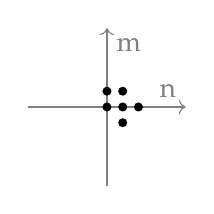
\begin{tikzpicture}[scale=.2]
\draw[thin, gray, ->] (0,-5) -- (0,5) node[anchor=north west] {m};
\draw[thin, gray, ->] (-5,0) -- (5,0) node[anchor=south east] {n};
\foreach \x in {-4,-3,-2,-1,1,2,3,4}
\draw[thin, gray] (\x,2pt) -- (\x,-2pt);
\foreach \y in {-4,-3,-2,-1,1,2,3,4}
\draw[thin, gray] (2pt,\y) -- (-2pt,\y);

\node[draw,circle,inner sep=1pt,fill] at (0,0) {};
\node[draw,circle,inner sep=1pt,fill] at (1,0) {};
\node[draw,circle,inner sep=1pt,fill] at (0,1) {};
\node[draw,circle,inner sep=1pt,fill] at (1,1) {};
\node[draw,circle,inner sep=1pt,fill] at (2,0) {};
\node[draw,circle,inner sep=1pt,fill] at (1,-1) {};
\end{tikzpicture}
$\qquad$
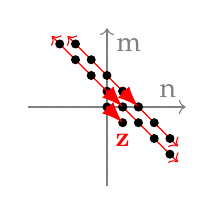
\begin{tikzpicture}[scale=.2]
\draw[thin, gray, ->] (0,-5) -- (0,5) node[anchor=north west] {m};
\draw[thin, gray, ->] (-5,0) -- (5,0) node[anchor=south east] {n};
\foreach \x in {-4,-3,-2,-1,1,2,3,4}
\draw[thin, gray] (\x,2pt) -- (\x,-2pt);
\foreach \y in {-4,-3,-2,-1,1,2,3,4}
\draw[thin, gray] (2pt,\y) -- (-2pt,\y);

\node[draw,circle,inner sep=1pt,fill] at (0,0) {};
\node[draw,circle,inner sep=1pt,fill] at (1,0) {};
\node[draw,circle,inner sep=1pt,fill] at (0,1) {};
\node[draw,circle,inner sep=1pt,fill] at (1,1) {};
\node[draw,circle,inner sep=1pt,fill] at (2,0) {};
\node[draw,circle,inner sep=1pt,fill] at (1,-1) {};

\draw [thin, red,-latex, <->] (-3.5,4.5) -- (4.5, -3.5) {};
\draw [thin, red,-latex, <->] (-2.5,4.5) -- (4.5, -2.5) {};

\foreach \x in {-3,-2,-1,1,2,3,4}
\node[draw,circle,inner sep=1pt,fill] at (\x,1 - \x) {};
\foreach \x in {-2,-1,0,1,2,3,4}
\node[draw,circle,inner sep=1pt,fill] at (\x,2 - \x) {};

\draw [ultra thick,-latex,red] (0,0) -- (1,-1) node [below] {$\zz$};
\draw [ultra thick,-latex,red] (0,1) -- (1,0) {};
\draw [ultra thick,-latex,red] (1,1) -- (2,0) {};
\end{tikzpicture}
$\qquad$
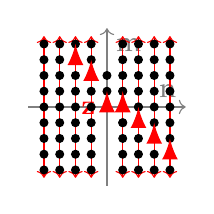
\begin{tikzpicture}[scale=.2]
\draw[thin, gray, ->] (0,-5) -- (0,5) node[anchor=north west] {m};
\draw[thin, gray, ->] (-5,0) -- (5,0) node[anchor=south east] {n};
\foreach \x in {-4,-3,-2,-1,1,2,3,4}
\draw[thin, gray] (\x,2pt) -- (\x,-2pt);
\foreach \y in {-4,-3,-2,-1,1,2,3,4}
\draw[thin, gray] (2pt,\y) -- (-2pt,\y);

\node[draw,circle,inner sep=1pt,fill] at (0,0) {};
\node[draw,circle,inner sep=1pt,fill] at (1,0) {};
\node[draw,circle,inner sep=1pt,fill] at (0,1) {};
\node[draw,circle,inner sep=1pt,fill] at (1,1) {};
\node[draw,circle,inner sep=1pt,fill] at (2,0) {};
\node[draw,circle,inner sep=1pt,fill] at (1,-1) {};

\draw [ultra thick,-latex,red] (0,0) -- (0,1) node [below left] {$\zz$};

\node[draw,circle,inner sep=1pt,fill] at (0,2) {};

\foreach \x in {-4,-3,-2,-1,1,2,3,4}
\draw [thin, red,-latex, <->] (\x, -4.5) -- (\x, 4.5) {};

\foreach \x in {-4,-3,-2,-1,1,2,3,4}
\foreach \y in {-4,-3,-2,-1,0,1,2,3,4}
\node[draw,circle,inner sep=1pt,fill] at (\x,\y) {};

\foreach \x in {-2,-1,1,2,3,4}
\draw [ultra thick,-latex,red] (\x,-\x + 1) -- (\x,-\x+2) {};
\end{tikzpicture}
$\cdots$\end{center}


\end{frame}


%%%%%%%%%%%%%%%%%%%%%%%%%%%%%%%%%%%%%%%%%%%%%%%%%%%%%%
%%%%%%%%%%%%%%%%%%%%%%%%%%%%%%%%%%%%%%%%%%%%%%%%%%%%%%
\begin{frame}{A $\cd(T^2)$-Action on $\cd(D^2 \times S^1)$}

\begin{theorem}[P.]
The $\cd(T^2)$-action on $\cd(D^2 \times S^1)$ is determined by the equations
\begin{align*}
    \widetilde{P}_{1,0} \cdot \widetilde{Q}_\lambda &= \Bigg(\langle \widetilde{P}_1 \rangle + \{1\} \Big( v^{-1}\sum_{\square\in\lambda} s^{2\cn(\square)} - v \sum_{\square\in\lambda} s^{-2\cn(\square)} \Big) \Bigg) \widetilde{Q}_\lambda \\
    \widetilde{P}_{2,0} \cdot \widetilde{Q}_\lambda &= \Bigg(\langle \widetilde{P}_2 \rangle + \{2\} \Big( v^{-2}\sum_{\square\in\lambda} s^{4\cn(\square)} - v^2 \sum_{\square\in\lambda} s^{-4\cn(\square)} \Big) \Bigg) \widetilde{Q}_\lambda \\
    \widetilde{P}_{0,1} \cdot \widetilde{Q}_\lambda &= \sum_{\substack{\lambda \subset \mu \\ \mu = \lambda + \square}} \widetilde{Q}_\mu + \sum_{\substack{\nu \subset \lambda \\ \lambda = \nu + \square}} \widetilde{Q}_\nu \\
    \widetilde{P}_{1,1} \cdot \widetilde{Q}_\lambda &= v^{-1} \sum_{\substack{\lambda \subset \mu \\ \mu = \lambda + \square}} s^{2\cn(\square)} \widetilde{Q}_\mu + v \sum_{\substack{\nu \subset \lambda \\ \lambda = \nu + \square}} s^{-2\cn(\square)} \widetilde{Q}_\nu 
\end{align*}
\end{theorem}
\end{frame}


%%%%%%%%%%%%%%%%%%%%%%%%%%%%%%%%%%%%%%%%%%%%%%%%%%%%%%
%%%%%%%%%%%%%%%%%%%%%%%%%%%%%%%%%%%%%%%%%%%%%%%%%%%%%%
\section{\scshape Type B/C/D Schur Functions}
\begin{frame}{Symmetric Functions and $\ch(A)^+$}

\end{frame}

%%%%%%%%%%%%%%%%%%%%%%%%%%%%%%%%%%%%%%%%%%%%%%%%%%%%%%
%%%%%%%%%%%%%%%%%%%%%%%%%%%%%%%%%%%%%%%%%%%%%%%%%%%%%%
\begin{frame}{Frame 1}

\end{frame}

%%%%%%%%%%%%%%%%%%%%%%%%%%%%%%%%%%%%%%%%%%%%%%%%%%%%%%
%%%%%%%%%%%%%%%%%%%%%%%%%%%%%%%%%%%%%%%%%%%%%%%%%%%%%%
\begin{frame}{Frame 1}

\end{frame}

%%%%%%%%%%%%%%%%%%%%%%%%%%%%%%%%%%%%%%%%%%%%%%%%%%%%%%
%%%%%%%%%%%%%%%%%%%%%%%%%%%%%%%%%%%%%%%%%%%%%%%%%%%%%%
\begin{frame}{Frame 1}

\end{frame}

\end{document}